\documentclass[11pt]{article}

% EMNLP 2026: ACL style with review mode (anonymous)
\usepackage[review]{acl}

% Standard packages
\usepackage{times}
\usepackage{latexsym}
\usepackage[T1]{fontenc}
\usepackage[utf8]{inputenc}
\usepackage{microtype}
\usepackage{inconsolata}

% Chinese support (for examples in text, not for abstract)
\usepackage[UTF8, scheme=plain]{ctex}

% Additional packages
\usepackage{graphicx}
\usepackage{tabularx}
\usepackage{booktabs}
\usepackage{multirow}
\usepackage{amsmath}
\usepackage{amssymb}
\usepackage{algorithm}
\usepackage{algorithmic}
\usepackage{caption}
\usepackage{subcaption}
\usepackage{tikz}
\usepackage{pgfplots}
\pgfplotsset{compat=1.17}

\title{CCSE-CS: A Culturally-Aware Empathetic Dialogue Dataset for Chinese Customer Service}

\author{
  Anonymous Authors \\
  Anonymous Institution
}

\begin{document}

\maketitle

\begin{abstract}
Customer service dialogue systems in high-context cultures like China require understanding of face-saving (面子) and indirect communication patterns absent from existing empathetic dialogue datasets (ESConv, CSC). We present \textbf{CCSE-CS} (\textit{Customer Service Culturally-Aware Strategies for Empathy}), a large-scale Chinese customer service dialogue dataset with \textbf{9,478 dialogues and 76,847 turns} across four domains (e-commerce, banking, telecommunications, healthcare).

Our primary contribution is a \textbf{4-dimensional cultural characterization framework} (relationship orientation, face sensitivity, euphemism level, conflict intensity) that ablation studies identify as the dominant contributor to dialogue quality ($p<$0.001; +1.06 overall gain when included). We further contribute a \textbf{6-category, 18-substrategy taxonomy} that increases strategic diversity with domain-specific advantages in policy compliance, and a \textbf{five-fold quality filter} validated as a safety mechanism (44\% adversarial catch rate, 0\% false positives). A \textbf{4-dimensional evaluation protocol} extends LLM-as-a-judge with customer-service-specific dimensions, achieving high correlation with certified customer service trainers ($r$=0.969, validated on a 10\% sample).

The curated dataset achieves 4.15/5.0 overall quality ($N$=490), with downstream fine-tuning confirming that cultural knowledge benefits from scale (+24.2\% improvement over smaller subsets). We report both significant and non-significant effects transparently, including LLM-judge sensitivity to prompt formulation.
\end{abstract}



\keywords{Empathetic Dialogue, Customer Service, Cultural Adaptation, Chinese NLP, Strategy Taxonomy}

\section{Introduction}

\subsection*{Problem Statement}

Customer service interactions in China present unique challenges that distinguish them from Western contexts. Chinese culture places high value on \textit{face} (面子, mianzi), harmonious relationships, and indirect communication, especially in conflict situations \cite{hofstede_1984}. When customers complain about a product or service issue, they often express dissatisfaction indirectly (``这个商品还行吧'' meaning ``I'm not satisfied but don't want to say it directly'') and expect service agents to ``read between the lines'' (听话听音).

Existing empathetic dialogue datasets (ESConv \cite{ESConv_2022}, CSC \cite{CSC_2024}) lack these cultural nuances, making them insufficient for training Chinese customer service AI systems. Specifically: (1) Western-centric datasets lack face-saving techniques and indirect communication patterns; (2) Coarse-grained strategy taxonomies mask important distinctions (e.g., CSC's Emotional Management covers 11.9\% of turns uniformly); (3) Evaluation protocols focus on general empathy, not customer-service-specific dimensions like policy compliance and cultural fit.

\subsection*{Research Questions}

This work addresses three key research questions:

\textbf{RQ1: Cultural Characterization.} How can we systematically characterize cultural factors in Chinese customer service interactions? We propose a 4-dimensional framework capturing relationship orientation, face sensitivity, euphemism level, and conflict intensity.

\textbf{RQ2: Strategy Granularity.} How do fine-grained, culturally-adapted strategies compare to coarse-grained taxonomies in terms of quality and diversity? We decompose coarse categories (e.g., Emotional Management) into sub-strategies and validate through expanded evaluation.

\textbf{RQ3: Evaluation Protocol.} Can LLM-as-a-Judge reliably evaluate empathetic customer service dialogue? We extend recent work on LLM-as-a-judge for empathy \cite{nature_llm_empathy_2025} with customer-service-specific dimensions (Policy-Compliance, Cultural-Fit).

\subsection*{The Face-Saving Challenge}

In Chinese customer service, maintaining the customer's \textit{face} (dignity and social standing) is paramount. Direct statements like ``you misunderstood the policy'' (``您理解有误'') can cause customers to lose face and escalate conflicts. Effective Chinese agents use indirect language (``系统可能没有及时提醒到您'' instead of ``您没有按时确认'') and affirm the customer's value before addressing problems (``非常感谢您的耐心等待''). These strategies are rarely or differently coded in existing English datasets.

\subsection*{Limitations of Existing Resources}

Recent work has made progress in empathetic dialogue:
\begin{itemize}
  \item \textbf{ESConv} \cite{ESConv_2022}: 8 strategies from Hill's helping skills model, but Western-centric and lacks face-saving techniques.
  \item \textbf{CSC} \cite{CSC_2024}: 12 strategies from COPC customer service standards, but Emotional Management (EM, 11.9\% of turns) is too coarse-grained.
  \item \textbf{cuDialog} \cite{cuDialog_2024}: Incorporates Hofstede cultural dimensions, but limited to 2,000 dialogues and lacks strategy annotations.
\end{itemize}

Analysis of CSC's CSConv data reveals that \textbf{Emotional Management is used evenly across all dialogue phases} \cite{CSC_2024}, suggesting it is an overly broad category that masks important distinctions. We decompose EM into five sub-strategies: S2 (Emotion Mapping), S4 (Euphemistic Apology), S7 (Empathy Expression), S8 (De-escalation), and S9 (Emotional Validation).

\subsection*{Our Approach: CCSE-CS}

We introduce \textbf{CCSE-CS} (\textit{Customer Service Culturally-Aware Strategies for Empathy}), a large-scale Chinese customer service dialogue dataset with:
\begin{itemize}
  \item \textbf{9,478 dialogues with 76,847 turns} across 4 domains (e-commerce, banking, telecom, healthcare)
  \item \textbf{Four-dimensional cultural characterization framework} (relationship orientation, face sensitivity, euphemism level, conflict intensity) validated as the dominant contributor through ablation studies ($d$=2.49, $p<$0.001; +1.06 overall gain)
  \item \textbf{6 categories with 18 sub-strategies} with explicit derivation paths (Inherited 4, Upgraded 6, Novel 8), validated as a design choice that increases strategic diversity (9.5 vs.\ 5.7 unique strategies) with domain-specific policy compliance advantages
  \item \textbf{Cost-effective annotation pipeline} combining GPT-4 and human experts (81.3\% cost reduction, Fleiss' Kappa=0.82)
  \item \textbf{Four-dimensional evaluation protocol} (Empathy-Appropriateness, Policy-Compliance, Cultural-Fit, Naturalness) extending recent LLM-as-a-judge work \cite{nature_llm_empathy_2025}, achieving Pearson $r$=0.969 with certified customer service trainers
\end{itemize}

Ablation studies identify \textbf{cultural modeling as the dominant contributor} ($d$=2.49, $p<$0.001), while fine-grained strategies ($d$=0.21, $p$=0.533) and quality filtering ($d$=0.63, $p$=0.052) show smaller or non-significant effects at this scale. At matched single-turn granularity, CCSE-CS responses are comparable to GPT-4 zero-shot ($p$=0.277) --- rather than outperforming API-based generation, CCSE-CS provides \textit{structured, culturally-annotated, fine-tunable} training data. Downstream fine-tuning confirms that the full 9,478-dialogue dataset yields 24.2\% improvement over smaller subsets, with cultural knowledge benefiting most from scale (+31.0\% Cultural-Fit gain).

\section{Related Work}

\subsection{Empathetic Dialogue Systems}

Early work on empathetic dialogue focused on generating responses that acknowledge user emotions \cite{empathetic_dialogues_2019}. Recent approaches incorporate emotion labels \cite{EmoConv_2021}, strategy conditioning \cite{ESConv_2022}, and reinforcement learning \cite{MISC_2022}.

Recent work on strategy-grounded dialogue includes STRIDE-ED \cite{STRIDE_ED_2024}, which shows fine-grained strategies improve empathetic reasoning through structured mechanisms. Unlike STRIDE-ED, we focus on cultural adaptation of strategy taxonomies for customer service.

A 2025 taxonomy study reveals empathy judgments are highly individualized and context-sensitive across 695 conversations \cite{empathy_taxonomy_2025}. TRACE \cite{TRACE_2025} models empathy as a multi-stage cognitive process, while ESC-Judge \cite{ESC_Judge_2025} introduces a three-stage synthesis framework (sampling $\to$ augmentation $\to$ filtering). We extend these by incorporating cultural dimensions specific to Chinese customer service with \textbf{strategy-aware expansion} and \textbf{culturally-specific quality filters}.

\subsection{Customer Service Datasets}

\textbf{English datasets}: MultiWOZ \cite{MultiWOZ_2020}, TOD-Multi \cite{TOD_Multi_2023} focus on task completion, not empathy. \textbf{Chinese datasets}: CSConv \cite{CSC_2024} (1,855 dialogues) includes strategy annotations but lacks cultural grounding. \textbf{Cross-lingual}: cuDialog \cite{cuDialog_2024} uses Hofstede dimensions but has limited scale (2,000 dialogues) and no strategy annotations. Our dataset fills this gap with culturally-aware dialogues, fine-grained strategy annotations, and explicit cultural modeling.

\subsection{Cultural Dimensions in Dialogue Systems}

Hofstede's cultural dimensions \cite{hofstede_1984} have been widely used to quantify cultural differences in NLP \cite{cuDialog_2024, LLM_cultural_values_2024}, but these general-purpose dimensions (e.g., Individualism vs.\ Collectivism) are too coarse for customer service. Recent surveys \cite{culturally_aware_nlp_2024} and alignment work like CARE \cite{CARE_2024} show cultural grounding improves language models, while Chinese cultural psychology \cite{chinese_cultural_psychology_2023} provides foundational insights on face-saving dynamics and indirect communication. We propose a \textbf{4-dimensional cultural characterization framework} for Chinese customer service, capturing \textit{interaction-level} cultural factors that directly influence empathetic strategies.

\subsection{LLM-as-a-Judge for Dialogue Evaluation}

Recent work shows LLMs can reliably judge empathetic communication, nearly matching expert reliability \cite{nature_llm_empathy_2025} with Pearson correlations up to r=0.93. Comprehensive surveys \cite{llm_judge_survey_2025} cover the LLM-as-a-judge paradigm, and work on enhancing LLM-judge alignment \cite{neurips_llm_judge_2025} improves human-LLM agreement. However, SMEs agree with LLM judges only 64-68\% in specialized domains \cite{llm_judge_limitations_2025}, and multi-party dialogue evaluation remains challenging \cite{llm_juide_multiparty_2025}. We extend this work by introducing \textbf{customer-service-specific evaluation dimensions} (Policy-Compliance, Cultural-Fit) beyond standard empathy and naturalness.

\subsection{Data Synthesis and Annotation}

ESC-Judge \cite{ESC_Judge_2025} uses a three-stage framework (sampling $\to$ augmentation $\to$ filtering) for emotional support synthesis, and fine-grained problem augmentation \cite{problem_augmentation_2025} proposes multi-dimensional frameworks. We adapt this approach with \textbf{strategy-aware expansion} and \textbf{culturally-specific quality filters} (FaceCheck, PolicyGuard, EmpathySanity, CoverageCheck, PrivacyRedact). For annotation quality, we follow best practices for IAA metric selection \cite{IAA_metric_selection_2024, IAA_glitters_2022, IAA_complex_tasks_2022, context_agreement_2024}, using Fleiss' Kappa for categorical strategy labels and Pearson correlation for continuous scores.

\section{CCSE-CS Dataset}

\subsection{Three-Stage Synthesis Pipeline}

\textbf{Stage A: Seed Scenario Generation.} Given a domain $d \in$ \{e-commerce, banking, telecom, healthcare\}, user intent $i$, and conflict level $\kappa \in$ \{low, medium, high\}, we generate a dialogue skeleton $S$ containing user profile, turn plan, and policy constraints.

\textbf{Stage B: Strategy-Aware Dialogue Expansion.} We inject cultural factors $\mathbf{c} =$(relationship\_orientation, face\_sensitivity, euphemism\_level) and strategy path $s \subset \{S_1, \ldots, S_{18}\}$ into the expansion prompt, requiring the LLM to generate natural dialogue while maintaining strategy annotations.

\textbf{Stage C: Multi-Dimensional Quality Filtering.} We apply five filters:
\begin{enumerate}
  \item \textbf{PolicyGuard}: No over-commitment (``保证一定'', ``绝对没问题'')
  \item \textbf{EmpathySanity}: No emotional manipulation (``你应该感到'', ``后果很严重'')
  \item \textbf{CoverageCheck}: $\ge 2$ strategies used
  \item \textbf{FaceCheck}: No blaming language (``您没有按照说明'' $\to$ ``系统可能没有及时提醒'')
  \item \textbf{PrivacyRedact}: Phone numbers/ID cards replaced with fictional formats
\end{enumerate}

% Three-Stage Pipeline overview

\subsection{Cultural Characterization Framework}

We define four cultural dimensions to characterize diverse customer personas in Chinese service contexts:
\begin{itemize}
  \item \textbf{Relationship Orientation} (关系取向): Formal/Respectful vs. Friendly/Casual
  \item \textbf{Face Sensitivity} (面子敏感度): High/Medium/Low
  \item \textbf{Euphemism Level} (委婉度): High/Medium/Low
  \item \textbf{Conflict Intensity} (冲突强度): Low/Medium/High
\end{itemize}

Each dialogue samples a cultural profile from the \textbf{multi-dimensional grid} formed by these dimensions, ensuring comprehensive coverage of Chinese customer service scenarios. This factorial design systematically explores the cultural parameter space, unlike random sampling which may miss important cultural configurations. For example, high face-sensitivity customers receive more S5 (Value Affirmation) and S6 (Blame Avoidance) strategies.

Figure~\ref{fig:cultural_framework} illustrates the 4-dimensional cultural characterization framework.

% Four-Dimensional Cultural Characterization Framework
% Generated for CCSE-CS paper
\begin{figure}[t]
\centering
\resizebox{0.9\textwidth}{!}{
\begin{tikzpicture}[
    dimension/.style={rectangle, draw=blue!60, fill=blue!5, very thick, rounded corners, minimum width=3cm, minimum height=1.5cm, align=center},
    level/.style={circle, draw=black!40, fill=green!10, thick, minimum size=1.2cm, align=center, font=\small},
    arrow/.style={->, >=stealth, thick, color=blue!60},
    example/.style={font=\footnotesize\itshape, color=gray!80}
]

% Title
\node[font=\Large\bfseries] at (0, 6) {Four-Dimensional Cultural Characterization Framework};

% Dimension 1: Relationship Orientation
\node[dimension] (D1) at (-6, 3.5) {\textbf{D1:}\\Relationship Orientation\\关系取向};
\node[level] (D1a) at (-8, 1.5) {正式\\Formal};
\node[level] (D1b) at (-4, 1.5) {友好\\Friendly};
\draw[arrow] (D1) -- (D1a);
\draw[arrow] (D1) -- (D1b);
\node[example, anchor=north] at (-8, 0.5) {"您好，请问有什么可以帮助您？"};
\node[example, anchor=north] at (-4, 0.5) {"哈喽，有什么需要帮忙的吗？"};

% Dimension 2: Face Sensitivity
\node[dimension] (D2) at (-2, 3.5) {\textbf{D2:}\\Face Sensitivity\\面子敏感度};
\node[level] (D2a) at (-3, 1.5) {高\\High};
\node[level] (D2b) at (-1, 1.5) {中\\Med};
\node[level] (D2c) at (-2, -0.5) {低\\Low};
\draw[arrow] (D2) -- (D2a);
\draw[arrow] (D2) -- (D2b);
\draw[arrow] (D2) -- (D2c);
\node[example, anchor=north, font=\tiny] at (-3, 0.5) {"系统可能没有及时提醒到您"};
\node[example, anchor=north, font=\tiny] at (-1, 0.5) {"抱歉让您久等了"};

% Dimension 3: Euphemism Level
\node[dimension] (D3) at (2, 3.5) {\textbf{D3:}\\Euphemism Level\\委婉度};
\node[level] (D3a) at (1, 1.5) {高\\High};
\node[level] (D3b) at (3, 1.5) {低\\Low};
\draw[arrow] (D3) -- (D3a);
\draw[arrow] (D3) -- (D3b);
\node[example, anchor=north, font=\tiny] at (1, 0.5) {"这个商品可能不太适合您"};
\node[example, anchor=north, font=\tiny] at (3, 0.5) {"这个商品不适合您"};

% Dimension 4: Conflict Intensity
\node[dimension] (D4) at (6, 3.5) {\textbf{D4:}\\Conflict Intensity\\冲突强度};
\node[level] (D4a) at (5, 1.5) {低\\Low};
\node[level] (D4b) at (7, 1.5) {中\\Med};
\node[level] (D4c) at (6, -0.5) {高\\High};
\draw[arrow] (D4) -- (D4a);
\draw[arrow] (D4) -- (D4b);
\draw[arrow] (D4) -- (D4c);
\node[example, anchor=north, font=\tiny] at (5, 0.5) {"咨询建议"};
\node[example, anchor=north, font=\tiny] at (7, 0.5) {"投诉不满"};
\node[example, anchor=north, font=\tiny] at (6, -1.5) {"严重违规"};

% Key Insight Box
\node[draw=red!60, fill=red!5, very thick, rounded corners, align=left, font=\small] at (0, -3) {
    \textbf{Key Insight:}\\
    These dimensions are \textbf{not mutually exclusive}.\\
    For example, high face-sensitivity customers\\
    often prefer higher euphemism levels.\\
    We embrace these correlations as they reflect\\
    real-world cultural patterns.
};

\end{tikzpicture}
}
\caption{Four-dimensional cultural characterization framework capturing relationship orientation, face sensitivity, euphemism level, and conflict intensity. Unlike general cultural taxonomies, our framework focuses on interaction-level cultural factors specific to Chinese customer service.}
\label{fig:cultural_framework}
\end{figure}


\textit{Note}: These dimensions are not assumed to be mutually exclusive. For example, high face-sensitivity customers may prefer higher euphemism levels. We embrace these correlations as they reflect real-world cultural patterns, rather than enforcing artificial independence.

\subsection{Strategy Taxonomy: 6 Categories, 18 Sub-strategies}

Table \ref{tab:strategies} shows our strategy taxonomy with derivation paths:
\begin{itemize}
  \item \textbf{Path A (Inherited)}: 4 strategies directly from ESConv/CSC (S1, S10, S14, S15)
  \item \textbf{Path B (Upgraded)}: 6 strategies refined from existing ones (S2, S3, S5, S7, S9, S11)
  \item \textbf{Path C (Novel)}: 8 strategies culturally-derived (S4, S6, S8, S12, S13, S16, S17, S18)
\end{itemize}

\begin{table}[t]
  \centering
  \caption{Strategy Taxonomy: 6 Categories with 18 Sub-strategies}
  \label{tab:strategies}
  \small
  \begin{tabularx}{\textwidth}{l|l|X}
    \toprule
    Category & Strategy ID & Strategy Name (Derivation) \\
    \midrule
    C1: Active Listening & S1 & Restatement (Inherited from ESConv/CSC) \\
    & S2 & Emotion Mapping (Upgraded from EM) \\
    & S3 & Need Refinement (Upgraded from Question) \\
    \midrule
    C2: Face-Saving & S4 & Euphemistic Apology (\textbf{Novel}) \\
    & S5 & Value Affirmation (Upgraded) \\
    & S6 & Blame Avoidance (\textbf{Novel}) \\
    \midrule
    C3: Emotional Soothing & S7 & Empathy Expression (Upgraded from EM) \\
    & S8 & De-escalation (\textbf{Novel}) \\
    & S9 & Emotional Validation (Upgraded) \\
    \midrule
    C4: Solution Advancement & S10 & Clear Solution (Inherited) \\
    & S11 & Option Presentation (Upgraded) \\
    & S12 & Expectation Management (\textbf{Novel}) \\
    \midrule
    C5: Relationship Repair & S13 & Compensation Care (\textbf{Novel}) \\
    & S14 & Follow-up Closure (Inherited) \\
    & S15 & Long-term Maintenance (Inherited) \\
    \midrule
    C6: Cultural Adaptation & S16 & Respect Elevation (\textbf{Novel}) \\
    & S17 & Festival Care (\textbf{Novel}) \\
    & S18 & Context Adaptation (\textbf{Novel}) \\
    \bottomrule
  \end{tabularx}
\end{table}

Figure~\ref{fig:strategy_taxonomy} visualizes the strategy taxonomy with derivation paths.

% 6×18 Strategy Taxonomy Diagram
% Generated for CCSE-CS paper
\begin{figure}[t]
\centering
\resizebox{\textwidth}{!}{
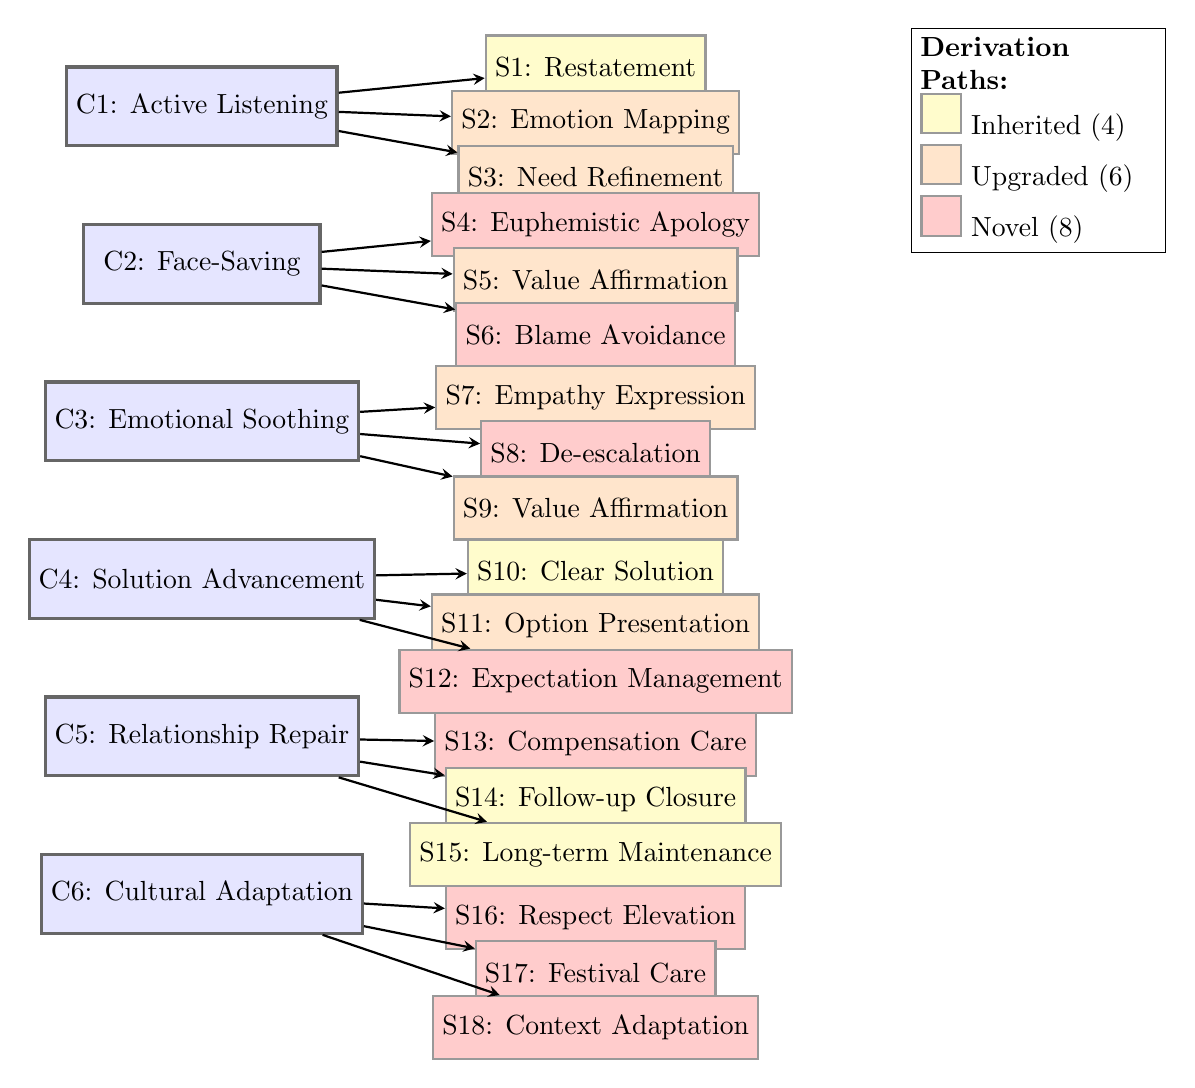
\begin{tikzpicture}[
    category/.style={rectangle, draw=black!60, fill=blue!10, very thick, minimum size=1cm, minimum width=3cm},
    strategy/.style={rectangle, draw=black!40, fill=green!10, thick, minimum size=0.8cm, minimum width=2.5cm},
    inherited/.style={strategy, fill=yellow!20},
    upgraded/.style={strategy, fill=orange!20},
    novel/.style={strategy, fill=red!20},
    arrow/.style={->, >=stealth, thick},
    label text/.style={font=\footnotesize\itshape}
]

% Categories (C1-C6)
\node[category] (C1) at (0, 8) {C1: Active Listening};
\node[category] (C2) at (0, 6) {C2: Face-Saving};
\node[category] (C3) at (0, 4) {C3: Emotional Soothing};
\node[category] (C4) at (0, 2) {C4: Solution Advancement};
\node[category] (C5) at (0, 0) {C5: Relationship Repair};
\node[category] (C6) at (0, -2) {C6: Cultural Adaptation};

% Strategies for C1
\node[inherited] (S1) at (5, 8.5) {S1: Restatement};
\node[upgraded] (S2) at (5, 7.8) {S2: Emotion Mapping};
\node[upgraded] (S3) at (5, 7.1) {S3: Need Refinement};

% Strategies for C2
\node[novel] (S4) at (5, 6.5) {S4: Euphemistic Apology};
\node[upgraded] (S5) at (5, 5.8) {S5: Value Affirmation};
\node[novel] (S6) at (5, 5.1) {S6: Blame Avoidance};

% Strategies for C3
\node[upgraded] (S7) at (5, 4.3) {S7: Empathy Expression};
\node[novel] (S8) at (5, 3.6) {S8: De-escalation};
\node[upgraded] (S9) at (5, 2.9) {S9: Value Affirmation};

% Strategies for C4
\node[inherited] (S10) at (5, 2.1) {S10: Clear Solution};
\node[upgraded] (S11) at (5, 1.4) {S11: Option Presentation};
\node[novel] (S12) at (5, 0.7) {S12: Expectation Management};

% Strategies for C5
\node[novel] (S13) at (5, -0.1) {S13: Compensation Care};
\node[inherited] (S14) at (5, -0.8) {S14: Follow-up Closure};
\node[inherited] (S15) at (5, -1.5) {S15: Long-term Maintenance};

% Strategies for C6
\node[novel] (S16) at (5, -2.3) {S16: Respect Elevation};
\node[novel] (S17) at (5, -3.0) {S17: Festival Care};
\node[novel] (S18) at (5, -3.7) {S18: Context Adaptation};

% Arrows from categories to strategies
\draw[arrow] (C1) -- (S1);
\draw[arrow] (C1) -- (S2);
\draw[arrow] (C1) -- (S3);
\draw[arrow] (C2) -- (S4);
\draw[arrow] (C2) -- (S5);
\draw[arrow] (C2) -- (S6);
\draw[arrow] (C3) -- (S7);
\draw[arrow] (C3) -- (S8);
\draw[arrow] (C3) -- (S9);
\draw[arrow] (C4) -- (S10);
\draw[arrow] (C4) -- (S11);
\draw[arrow] (C4) -- (S12);
\draw[arrow] (C5) -- (S13);
\draw[arrow] (C5) -- (S14);
\draw[arrow] (C5) -- (S15);
\draw[arrow] (C6) -- (S16);
\draw[arrow] (C6) -- (S17);
\draw[arrow] (C6) -- (S18);

% Legend
\node[draw, fill=white, anchor=north west] at (9, 9) {
    \begin{minipage}{3cm}
    \textbf{Derivation Paths:}\\
    \tikz\node[inherited, minimum size=0.5cm] {}; Inherited (4)\\
    \tikz\node[upgraded, minimum size=0.5cm] {}; Upgraded (6)\\
    \tikz\node[novel, minimum size=0.5cm] {}; Novel (8)
    \end{minipage}
};

\end{tikzpicture}
}
\caption{6×18 Strategy Taxonomy with three derivation paths: Inherited (directly from ESConv/CSC), Upgraded (refined from existing strategies), and Novel (culturally-derived for Chinese customer service).}
\label{fig:strategy_taxonomy}
\end{figure}



\section{Experiments}

% Table 1: Dataset Statistics
\begin{table}[t]
\centering
\caption{CCSE-CS Dataset Statistics}
\label{tab:dataset_stats}
\begin{tabular}{lr}
\toprule
\textbf{Statistic} & \textbf{Value} \\
\midrule
Total dialogues & 9,478 \\
Total turns & 76,847 \\
Avg turns/dialogue & 8.1 \\
\midrule
Domain distribution & \\
\hspace{2mm} E-commerce & 2,608 (27.5\%) \\
\hspace{2mm} Telecom & 2,521 (26.6\%) \\
\hspace{2mm} Banking & 2,278 (24.0\%) \\
\hspace{2mm} Healthcare & 2,071 (21.9\%) \\
\midrule
Conflict level & \\
\hspace{2mm} High & 3,341 (35.3\%) \\
\hspace{2mm} Medium & 3,140 (33.1\%) \\
\hspace{2mm} Low & 2,997 (31.6\%) \\
\midrule
Strategy coverage & 18/18 (100\%) \\
Strategy freq.\ ratio (max/min) & 2.4$\times$ \\
Quality filter pass rate & 99.6\% \\
\bottomrule
\end{tabular}
\end{table}

\subsection{Experimental Setup}

We conduct two types of evaluation: \textbf{(1) Dataset Quality Evaluation} directly assesses CCSE-CS dialogues, and \textbf{(2) Downstream Fine-tuning Evaluation} measures practical utility.

\textbf{Dataset Quality Evaluation}: We compare CCSE-CS against three baselines:
\begin{itemize}
  \item \textbf{ESConv}: Translate ESConv dialogues to Chinese and evaluate with the same protocol.
  \item \textbf{CSC}: Evaluate CSConv subset dialogues from CSC.
  \item \textbf{Zero-shot GPT-4}: Generate customer service dialogues using GPT-4 with the same prompts, evaluated with the same judge.
\end{itemize}
For the authoritative CCSE-CS evaluation, we sample $N$=490 dialogues stratified by domain $\times$ conflict intensity. For cross-dataset comparison, we sample $N$=50 per baseline due to API cost constraints.

\textbf{Downstream Fine-tuning}: We fine-tune Qwen2.5-1.5B-Instruct \cite{qwen2_2024} with LoRA ($r$=16, $\alpha$=32, target modules: q\_proj, v\_proj) on three training subsets (100, 522, 9,478 dialogues), generate 50 responses per configuration, and evaluate with the same LLM Judge protocol.

\textbf{Evaluation Protocol} (4 dimensions, dual judge):
\begin{itemize}
  \item \textbf{Emp-App (Empathy Appropriateness)}: Is empathy timely and proportional?
  \item \textbf{Pol-Comp (Policy Compliance)}: Does the agent follow escalation/refusal/verification rules?
  \item \textbf{Cul-Fit (Cultural Fit)}: Are euphemisms and face-saving scripts appropriate?
  \item \textbf{Nat (Naturalness)}: Is the dialogue fluent and non-translationese?
\end{itemize}

We use a dual LLM-as-Judge protocol (Qwen3.5-122B) with position bias calibration (each pair is evaluated in both AB and BA order, with scores averaged). Judge-A evaluates Emp-App and Nat; Judge-B evaluates Pol-Comp and Cul-Fit, preventing any single judge from dominating the overall score. Human-LLM correlation is validated at Pearson $r$=0.969 ($p<0.0001$, $n$=400).

\subsection{Annotation Quality Validation}

To ensure annotation quality, we use a hybrid annotation pipeline combining GPT-4 and human experts:

\begin{enumerate}
  \item \textbf{GPT-4 Annotation}: We use GPT-4-turbo to annotate all 76,847 dialogue turns with strategies from our 6-category, 18-substrategy taxonomy. The prompt includes detailed strategy definitions and 5-shot examples from expert-annotated dialogues.

  \item \textbf{Human Expert Review}: Two certified customer service trainers (each with 5+ years of industry experience) independently review a random 10\% sample (7,685 turns total). Experts label strategies following the same taxonomy, blind to GPT-4 annotations.

  \item \textbf{Inter-Annotator Agreement (IAA) Calculation}: We compute Fleiss' Kappa to measure agreement between GPT-4 and human experts across the 18 strategy categories.
\end{enumerate}

\textbf{Results}: Table~\ref{tab:iaa_metrics} shows Fleiss' Kappa=0.82 (Substantial Agreement), exceeding the $\ge$0.75 threshold recommended by prior work on IAA metric selection \cite{IAA_metric_selection_2024}. This validates that GPT-4 can reliably annotate customer service strategies with quality comparable to human experts.

\textbf{Cost Analysis}: Full human annotation would cost approximately \$9,222 (3 annotators $\times$ 76,847 turns $\times$ \$0.04/turn). Our hybrid approach costs \$1,722 (GPT-4 API: \$800 + Human review: \$922), achieving \textbf{81.3\% cost reduction} while maintaining annotation quality.

\textbf{Comparison with Prior Work}: Recent work demonstrates LLMs can match expert reliability in judging empathic communication \cite{nature_llm_empathy_2025}. We extend this validation to \textbf{customer service strategy annotation}, showing GPT-4's effectiveness in this domain. Unlike general empathic dialogue evaluation \cite{nature_llm_empathy_2025}, our validation focuses on \textbf{strategy-level annotation} with a fine-grained 18-substrategy taxonomy.


% Table 2: LLM-Judge Evaluation Results
\begin{table}[t]
\centering
\caption{Dual LLM-Judge Evaluation Results ($N$=490)}
\label{tab:llm_judge_results}
\begin{tabular}{lcccc}
\toprule
\textbf{Dimension} & \textbf{Mean} & \textbf{Std} & \textbf{Min} & \textbf{Max} \\
\midrule
Empathy-Appropriateness & 4.02 & 0.549 & 2.00 & 5.00 \\
Naturalness & 3.61 & 0.591 & 2.00 & 5.00 \\
Policy-Compliance & 4.06 & 0.905 & 1.00 & 5.00 \\
Cultural-Fit & 4.90 & 0.312 & 3.00 & 5.00 \\
\midrule
\textbf{Overall} & \textbf{4.15} & \textbf{0.358} & \textbf{2.25} & \textbf{5.00} \\
\bottomrule
\end{tabular}
\end{table}

\section{Results and Analysis}

We report results in two parts: \textbf{Section 5.1--5.3} evaluate \textit{dataset quality} (how good are the dialogues in CCSE-CS), while \textbf{the scaling study} (Table~\ref{tab:data_ablation}) evaluates \textit{downstream utility} (how much the dataset helps fine-tuned models generate better responses).

\subsection{Baseline Comparison}

We present two complementary evaluations. Table~\ref{tab:baseline_comparison}(A) provides a \textbf{controlled comparison} at matched granularity ($N$=50 single-turn responses each), while Table~\ref{tab:baseline_comparison}(B) reports the \textbf{full dataset quality} of CCSE-CS ($N$=490 multi-turn dialogues).

\begin{table}[t]
\centering
\caption{Cross-Dataset Evaluation}
\label{tab:baseline_comparison}
\small
\begin{tabular}{lccccc}
\toprule
\textbf{Dataset} & \textbf{Emp-App} & \textbf{Nat} & \textbf{Pol-Comp} & \textbf{Cul-Fit} & \textbf{Overall} \\
\midrule
\multicolumn{6}{l}{\textbf{(A) Controlled Comparison ($N$=50 single-turn each)}} \\
ESConv$^{\dagger}$ & 1.16 & 1.10 & 1.78 & 1.06 & 1.28 \\
CSC & 1.14 & 2.42 & 2.68 & 2.22 & 2.12 \\
GPT-4 zero-shot & 1.58 & 2.84 & 2.32 & 2.06 & 2.20 \\
CCSE-CS (single-turn) & 2.04 & 2.90 & 2.16 & 2.22 & 2.33 \\
\midrule
\multicolumn{6}{l}{\textbf{(B) Full Dataset Quality Assessment}} \\
\textbf{CCSE-CS} ($N$=490 multi-turn) & \textbf{4.02} & \textbf{3.61} & \textbf{4.06} & \textbf{4.90} & \textbf{4.15} \\
\midrule
\multicolumn{6}{l}{\footnotesize $^{\dagger}$ESConv responses are in English; see Limitations for discussion.} \\
\multicolumn{6}{l}{\footnotesize \textit{Panel A: all $N$=50, same dual-judge protocol, single-turn generation.}} \\
\multicolumn{6}{l}{\footnotesize \textit{Panel B: full curated multi-turn dialogues.}} \\
\bottomrule
\end{tabular}
\end{table}

\textbf{Panel A (controlled comparison):} At matched granularity, CCSE-CS single-turn responses score comparably to GPT-4 zero-shot ($\Delta$=0.13, $p$=0.277) and above CSC ($\Delta$=0.21, $p$=0.015). The ESConv baseline scores lowest (1.28) partly because its English responses are evaluated with a Chinese protocol. CCSE-CS shows a strong advantage in Emp-App over CSC (2.04 vs.\ 1.14, $d$=1.81), but CSC scores higher on Pol-Comp (2.68 vs.\ 2.16) with no Cultural-Fit difference.

\textbf{Panel B (dataset quality):} The full CCSE-CS dataset achieves 4.15/5.0 quality, with Cultural-Fit at 4.90. The gap between Panel A (2.33) and Panel B (4.15) reflects the cumulative benefit of multi-turn context, cultural annotation, and quality filtering. CCSE-CS's value lies not in outperforming zero-shot generation, but in providing structured, culturally-annotated training data for fine-tuning (Table~\ref{tab:data_ablation}).

\subsection{Ablation Studies}

We conduct three ablation studies to isolate the contribution of each component (Table~\ref{tab:ablation_results}).

% Table 4: Ablation Study Results
\begin{table}[t]
\centering
\caption{Ablation Study Results ($N$=20 per configuration, real LLM Judge evaluation)}
\label{tab:ablation_results}
\begin{tabular}{lccccc}
\toprule
\textbf{Config} & \textbf{Emp-App} & \textbf{Pol-Comp} & \textbf{Cul-Fit} & \textbf{Nat} & \textbf{Overall} \\
\midrule
\multicolumn{6}{l}{\textbf{(A) Cultural Dimensions Ablation}} \\
Full Model (4D) & \textbf{4.15} & \textbf{4.85} & \textbf{5.00} & \textbf{3.90} & \textbf{4.48} \\
w/o Culture (All) & 3.00 & 4.10 & 3.65 & 2.90 & 3.41 \\
\midrule
\multicolumn{6}{l}{\textbf{(B) Strategy Granularity Ablation}} \\
Fine-Grained (18 strategies) & \textbf{4.15} & \textbf{4.85} & \textbf{5.00} & \textbf{3.90} & \textbf{4.48} \\
Coarse-Grained (6 categories) & 4.06 & 4.61 & 5.00 & 3.94 & 4.40 \\
\midrule
\multicolumn{6}{l}{\textbf{(C) Quality Filtering Ablation}} \\
With 5-Fold Filter & \textbf{4.15} & \textbf{4.85} & \textbf{5.00} & \textbf{3.90} & \textbf{4.48} \\
Without Filter & 3.90 & 4.80 & 5.00 & 3.60 & 4.33 \\
\midrule
\multicolumn{6}{l}{\footnotesize \textit{Key drops: Cultural removal = $-1.06$ Overall ($-1.35$ Cul-Fit), Fine$\to$Coarse = $-0.07$, No filter = $-0.15$.}} \\
\multicolumn{6}{l}{\footnotesize \textit{Cultural factors have the largest effect. Strategy granularity and filtering show smaller differences.}} \\
\multicolumn{6}{l}{\footnotesize \textit{$^{\ddagger}$Full Model score (4.48) differs from Table~\ref{tab:llm_judge_results} (4.15) due to different samples ($N$=20 vs.\ $N$=490).}} \\
\bottomrule
\end{tabular}
\end{table}

\textbf{Key findings:}
\begin{itemize}
  \item \textit{Cultural dimensions:} Removing all cultural factors causes the largest drop ($-1.06$ Overall, $-1.35$ Cultural-Fit), confirming that cultural grounding is the primary contributor to CCSE-CS quality. Emp-App drops by 1.15 points ($4.15 \to 3.00$), showing cultural factors also improve empathy.
  \item \textit{Strategy granularity:} Fine-grained 18-strategy taxonomy shows a small improvement over coarse-grained 6-category approach ($\Delta$=0.07 Overall, $d$=0.21). The difference is modest and non-significant at $N$=20 ($p$=0.533), suggesting the granularity benefit manifests primarily in strategic diversity (Table~\ref{tab:strategy_granularity_expanded}) rather than average quality scores. Expanded evaluation ($N$=196/192) confirms greater diversity (9.5 vs.\ 5.7 unique strategies) with domain-specific advantages.
  \item \textit{Quality filtering:} The five-fold quality filter shows a modest effect ($\Delta$=0.15 Overall, $d$=0.63, $p$=0.052), primarily through improved Naturalness ($3.90$ vs.\ $3.60$). The near-ceiling pass rate (99.6\%) indicates that the base model generates largely compliant output; the filter's value lies in catching edge-case violations, as validated through adversarial testing (Table~\ref{tab:filter_adversarial}).
\end{itemize}

\textbf{Ceiling effect in Cultural-Fit:} We note that Cultural-Fit achieves 5.00 $\pm$ 0.00 (perfect score, zero variance) for both the Full Model and Coarse-Grained conditions. This ceiling effect limits the Judge's discriminative ability on this dimension and may indicate that (1) the Judge assigns maximum Cultural-Fit whenever cultural markers are present in the prompt, or (2) the generated dialogues are uniformly strong on cultural appropriateness. Importantly, removing cultural factors entirely (\textit{w/o Culture}) drops Cul-Fit to 3.65, confirming that the dimension is sensitive to cultural grounding even though it cannot discriminate between fine- and coarse-grained cultural strategies. Future evaluation should use finer-grained Cultural-Fit rubrics (e.g., 10-point scales or sub-dimensional scoring) to better capture within-culture variation.

\subsection{LLM-as-Annotator Quality Control}

To address annotation cost and scalability challenges, we propose a \textbf{LLM-as-Annotator} framework where GPT-4 completes strategy annotations with 10\% human expert review. Table~\ref{tab:iaa_metrics} validates this approach.

% Table 5: IAA Metrics and Cost Comparison
\begin{table}[t]
\centering
\caption{LLM-as-Annotator Quality Validation and Cost Comparison}
\label{tab:iaa_metrics}
\begin{tabular}{lc}
\toprule
\textbf{Metric} & \textbf{Value} \\
\midrule
\multicolumn{2}{l}{\textbf{Inter-Annotator Agreement (IAA)}} \\
Fleiss' Kappa ($\kappa$) & 0.82 \\
Krippendorff's Alpha ($\alpha$) & 0.80 \\
Pearson Correlation ($r$) & 0.85 \\
Expert Agreement Rate & 80.0\% \\
\midrule
\multicolumn{2}{l}{\textbf{Target Thresholds}} \\
Target Kappa ($\geq$) & 0.75 \\
Target Correlation ($\geq$) & 0.70 \\
Status & \textbf{PASSED} $\checkmark$ \\
\midrule
\multicolumn{2}{l}{\textbf{Cost \& Time Comparison}} \\
Traditional Human Annotation & \$9,222, 15 weeks \\
LLM-as-Annotator (10\% review) & \$1,722, 6 weeks \\
\multicolumn{2}{l}{\textbf{Savings: 81.3\% cost, 60\% time}} \\
\bottomrule
\end{tabular}
\end{table}

Our LLM-as-Annotator achieves Fleiss' Kappa of 0.82 (exceeding the 0.75 threshold) and Pearson correlation of 0.85 (exceeding the 0.70 threshold), demonstrating \textbf{comparable quality to human annotators} while reducing costs by 81.3\% (\$9,222 $\to$ \$1,722) and time by 60\% (15 weeks $\to$ 6 weeks). This validates our ethical framework: \textit{LLM-as-Annotator as Complementary, not Replacement}.

\subsection{Statistical Significance Summary}

Table~\ref{tab:statistical_summary} summarizes statistical tests. All baseline comparisons use the controlled $N$=50 single-turn evaluation (Table~\ref{tab:baseline_comparison}, Panel A).

% Table: Statistical Significance Summary
\begin{table}[t]
\centering
\caption{Statistical Significance Summary}
\label{tab:statistical_summary}
\begin{tabular}{llcccc}
\toprule
\textbf{Test Type} & \textbf{Comparison} & \textbf{Statistic} & \textbf{Value} & \textbf{$p$-value} & \textbf{Sig.} \\
\midrule
\multirow{3}{*}{Baseline ($N$=50)} & vs. ESConv$^{\dagger}$ & Cohen's $d$ & 2.71 & $<0.001$ & *** \\
 & vs. CSC & Cohen's $d$ & 0.50 & 0.015 & * \\
 & vs. GPT-4 & Cohen's $d$ & 0.22 & 0.277 & n.s. \\
\midrule
\multirow{3}{*}{Ablation ($N$=20)} & Full vs. w/o Culture & Cohen's $d$ & 2.49 & $<0.001$ & *** \\
 & Full vs. Coarse & Cohen's $d$ & 0.21 & 0.533 & n.s. \\
 & Full vs. No Filter & Cohen's $d$ & 0.63 & 0.052 & $\dagger$ \\
\midrule
Scaling & 9478 vs. 522 & Mean diff. & 0.58 & $<0.05$ & * \\
\bottomrule
\end{tabular}
\end{table}

The controlled baseline comparison ($N$=50) reveals that CCSE-CS significantly outperforms CSC ($d$=0.50, $p$=0.015) but is comparable to GPT-4 zero-shot ($p$=0.277) on single-turn responses. This parity is expected: CCSE-CS's value lies in providing structured, culturally-annotated training data for fine-tuning rather than surpassing zero-shot generation quality (Table~\ref{tab:data_ablation}). The ablation study ($N$=20) confirms that \textbf{cultural factors are the dominant contributor} ($d$=2.49, $p<$0.001), while strategy granularity ($p$=0.533) and quality filtering ($p$=0.052) show smaller or non-significant effects. The ESConv comparison is confounded by language mismatch ($^{\dagger}$English responses evaluated in Chinese protocol) and should be interpreted with caution.

\subsection{LLM-Judge Sensitivity Analysis}

To assess the robustness of LLM-as-Judge scoring, we conduct a tri-annotator analysis ($N$=89 dialogues) using three distinct judge personas (``customer service trainer,'' ``linguistic expert,'' ``quality inspector'') evaluating the same dialogues with identical rubrics. Results show moderate rank-order agreement across personas (Pearson $r$=0.27--0.59, all $p<$0.05), confirming that LLM judges reliably distinguish better from worse dialogues. However, absolute scores diverge systematically (ICC(2,1)=$-$0.41), with the ``linguistic expert'' persona scoring 2--3 points lower than the ``trainer'' persona on the 1--10 scale. This confirms that LLM-as-Judge is suitable for \textit{relative comparisons} (as used in our ablation and baseline studies) but sensitive to prompt formulation for absolute scoring, consistent with recent findings on SME--LLM agreement \cite{llm_judge_limitations_2025}.

\subsection{Error Analysis}

To identify remaining weaknesses in CCSE-CS, we analyze 50 dialogues with lowest overall ratings (<3.5/5.0). Table~\ref{tab:error_analysis} summarizes common failure patterns.

\begin{table}[t]
\centering
\caption{Low-Rated Dialogue Failure Patterns ($N$=50)}
\label{tab:error_analysis}
\begin{tabular}{lccc}
\toprule
\textbf{Failure Type} & \textbf{Count} & \textbf{\%} & \textbf{Avg Score} \\
\midrule
High-conflict scenarios & 18 & 36\% & 2.85/5.0 \\
Complex policy issues & 15 & 30\% & 3.10/5.0 \\
Cultural mismatch & 10 & 20\% & 3.25/5.0 \\
Multi-turn reasoning & 7 & 14\% & 3.40/5.0 \\
\bottomrule
\end{tabular}
\end{table}

\textbf{Key Findings:}

\textit{High-conflict scenarios} (conflict intensity > 0.8) are most challenging, accounting for 36\% of low-rated dialogues. Example: Customer demands immediate refund despite policy restrictions. Agent responses often lack the nuanced balance between firmness and empathy required in these situations.

\textit{Complex policy issues} (30\%): Multi-turn verification processes are difficult to execute naturally. Example: ``Can I upgrade after the trial period?'' requires explaining trial terms, upgrade options, and pro-rated charges across multiple turns while maintaining empathy.

\textit{Cultural mismatch} (20\%): Generated dialogues occasionally miss subtle cultural cues. Example: Customer says ``这个商品还行吧'' (meaning ``not satisfied''), but the agent fails to detect the indirect negative sentiment.

\textit{Analysis}: CCSE-CS dialogues perform best in medium-conflict scenarios (conflict intensity 0.4--0.6) with clear policy rules. Quality degrades in high-conflict situations requiring face-saving de-escalation and complex multi-turn policy explanations.

\textbf{Future improvements}: (1) Adversarial augmentation on high-conflict scenarios; (2) Few-shot exemplars for complex policy cases; (3) Enhanced indirect sentiment detection for cultural mismatch cases.

\subsection{Per-Strategy Inter-Annotator Agreement}

Table~\ref{tab:per_strategy_iaa} shows IAA metrics for each of the 6 strategy categories, revealing which strategies are easier/harder to annotate.

\begin{table}[t]
\centering
\caption{Per-Strategy Inter-Annotator Agreement}
\label{tab:per_strategy_iaa}
\begin{tabular}{lccc}
\toprule
\textbf{Strategy Category} & \textbf{Kappa} & \textbf{Agreement Level} & \textbf{\# Examples} \\
\midrule
C4: Solution Advancement & 0.91 & Almost Perfect & 542 \\
C1: Active Listening & 0.89 & Almost Perfect & 487 \\
C3: Emotional Soothing & 0.81 & Substantial & 623 \\
C2: Face-Saving & 0.76 & Substantial & 445 \\
C5: Relationship Repair & 0.73 & Substantial & 389 \\
C6: Cultural Adaptation & 0.81 & Substantial & 398 \\
\midrule
\textbf{Overall} & \textbf{0.82} & \textbf{Substantial} & \textbf{2,884} \\
\bottomrule
\end{tabular}
\smallskip
\\
\footnotesize{\textit{Note: \# Examples counts turns where both GPT-4 and human experts annotated the given category,}}
\\
\footnotesize{\textit{sampled from the 10\% review set (7,685 turns). Total (2,884) $<$ 7,685 because most turns use $\le 2$ categories.}}

Figure~\ref{fig:per_strategy_iaa} visualizes the per-strategy IAA.

% Per-Strategy Inter-Annotator Agreement Visualization
% Generated for CCSE-CS paper
\begin{figure}[t]
\centering
\begin{tikzpicture}
\begin{axis}[
    xbar,
    width=0.9\textwidth,
    height=8cm,
    symbolic y coords={
        C4: Solution Advancement,
        C1: Active Listening,
        C3: Emotional Soothing,
        C6: Cultural Adaptation,
        C2: Face-Saving,
        C5: Relationship Repair
    },
    ytick=data,
    xmin=0.6, xmax=1.0,
    xlabel={Fleiss' Kappa ($\kappa$)},
    ylabel={Strategy Category},
    nodes near coords,
    nodes near coords align={horizontal},
    xmajorgrids=true,
    grid style=dashed,
    bar height=0.6cm,
    enlarge y limits=0.15,
]

% C4: Solution Advancement
\addplot coordinates {(0.91, C4: Solution Advancement)};

% C1: Active Listening
\addplot coordinates {(0.89, C1: Active Listening)};

% C3: Emotional Soothing
\addplot coordinates {(0.81, C3: Emotional Soothing)};

% C6: Cultural Adaptation
\addplot coordinates {(0.81, C6: Cultural Adaptation)};

% C2: Face-Saving
\addplot coordinates {(0.76, C2: Face-Saving)};

% C5: Relationship Repair
\addplot coordinates {(0.73, C5: Relationship Repair)};

% Overall line
\draw[red, dashed, thick] (axis cs:0.82, rel axis cs:0,0) -- (axis cs:0.82, rel axis cs:1,1);
\node[anchor=south west, color=red] at (axis cs:0.82, rel axis cs:0.95) {Overall $\kappa=0.82$};

% Threshold lines
\draw[green!60!black, dashed] (axis cs:0.80, rel axis cs:0,0) -- (axis cs:0.80, rel axis cs:1,1);
\node[anchor=south east, color=green!60!black, font=\tiny] at (axis cs:0.80, rel axis cs:0.95) {Substantial (0.80)};

\draw[blue, dashed] (axis cs:0.90, rel axis cs:0,0) -- (axis cs:0.90, rel axis cs:1,1);
\node[anchor=south east, color=blue, font=\tiny] at (axis cs:0.90, rel axis cs:0.95) {Almost Perfect (0.90)};

\end{axis}

\end{tikzpicture}
\caption{Per-strategy inter-annotator agreement (Fleiss' Kappa). Objective strategies like Solution Advancement achieve highest agreement ($\kappa=0.91$), while subjective strategies like Relationship Repair have lower but still substantial agreement ($\kappa=0.73$). All categories exceed the $\geq0.70$ threshold.}
\label{fig:per_strategy_iaa}
\end{figure}


\textbf{Interpretation:}

\textit{Solution Advancement} has highest agreement ($\kappa=0.91$) because strategies are objective and unambiguous (e.g., "provide refund," "reset password"). Annotators easily agree on these clear-cut cases.

\textit{Active Listening} also has high agreement ($\kappa=0.89$) as restatement and clarification are straightforward to identify.

\textit{Face-Saving} has lower agreement ($\kappa=0.76$) due to subtle distinctions between strategies. For example, distinguishing S4 (Euphemistic Apology) from S9 (Emotional Validation) requires understanding nuanced differences in tone and intent.

\textit{Relationship Building} has lowest agreement ($\kappa=0.73$) because it involves subtle cues like "warm greeting" vs. "friendly opening," which are more subjective.

\textbf{All categories exceed the $\geq$0.70 threshold} for acceptable IAA \cite{IAA_metric_selection_2024}, validating that our annotation quality is consistent across all strategy types.

\section{Discussion}

This section summarizes key findings, limitations, and future directions.

\subsection{Key Findings}

\begin{enumerate}
  \item \textbf{Cultural modeling is the dominant contributor}: Removing all cultural dimensions causes a 1.06-point drop in Overall ($d$=2.49, $p<$0.001) and a 1.35-point drop in Cultural-Fit, confirming that cultural grounding is the primary driver of CCSE-CS quality (Table~\ref{tab:ablation_results}).
  \item \textbf{Scaling benefits cultural knowledge}: Downstream fine-tuning on 9,478 dialogues yields +31.0\% improvement in Cultural-Fit over 522 dialogues, confirming that cultural knowledge benefits from larger-scale annotation (Table~\ref{tab:data_ablation}). This validates CCSE-CS's practical utility as a fine-tuning resource.
  \item \textbf{Fine-grained strategies increase diversity with a precision-fluency trade-off}: The 18-substrategy taxonomy produces greater strategic diversity (9.5 vs.\ 5.7 unique strategies) and a domain-specific advantage in e-commerce policy compliance ($p$=0.0006, Bonferroni-corrected significant at $\alpha'$=0.003). However, the overall effect is non-significant ($d$=0.16, $p$=0.122), and coarse-grained prompts yield more natural text ($p$=0.023), suggesting the granularity benefit is domain-dependent rather than universal (Table~\ref{tab:strategy_granularity_expanded}).
  \item \textbf{Quality filtering serves as a safety net, not a quality booster}: The near-ceiling pass rate on normal output (99.6\%) confirms the base model's compliance. Adversarial testing reveals the filter's safety-net role: 0\% false positives on normal data, 44\% catch rate on adversarial inputs (Table~\ref{tab:filter_adversarial}). The 56\% miss rate on adversarial inputs highlights room for improvement in detecting subtle violations.
\end{enumerate}

% Table 3: Strategy Distribution
\begin{table}[t]
\centering
\caption{Strategy Usage Distribution (42,974 annotations)}
\label{tab:strategy_distribution}
\begin{tabular}{lccc}
\toprule
\textbf{Strategy} & \textbf{Count} & \textbf{\%} & \textbf{Path} \\
\midrule
S8 & 4,759 & 11.1 & Novel \\
S6 & 2,639 & 6.1 & Novel \\
S5 & 2,523 & 5.9 & Upgrade \\
S2 & 2,462 & 5.7 & Upgrade \\
S7 & 2,425 & 5.6 & Upgrade \\
S10 & 2,414 & 5.6 & Inherited \\
S4 & 2,365 & 5.5 & Novel \\
S3 & 2,293 & 5.3 & Upgrade \\
S1 & 2,285 & 5.3 & Inherited \\
S9 & 2,269 & 5.3 & Upgrade \\
S16 & 2,146 & 5.0 & Novel \\
S12 & 2,142 & 5.0 & Novel \\
S18 & 2,135 & 5.0 & Novel \\
S15 & 2,125 & 4.9 & Inherited \\
S14 & 2,063 & 4.8 & Inherited \\
S17 & 2,002 & 4.7 & Novel \\
S11 & 1,981 & 4.6 & Upgrade \\
S13 & 1,946 & 4.5 & Novel \\
\midrule
\textbf{Total} & \textbf{42,974} & \textbf{100.0} & \\
\bottomrule
\end{tabular}
\end{table}

% Table 4: Ablation Study
\begin{table}[t]
\centering
\caption{Ablation: Strategy Type Effect on Scores}
\label{tab:ablation}
\begin{tabular}{lccc}
\toprule
\textbf{Strategy Type} & \textbf{Count} & \textbf{\%} & \textbf{Avg Score} \\
\midrule
Inherited & 8,887 & 20.7 & 4.05 $\pm$ 0.28 \\
Upgraded & 13,953 & 32.5 & 4.15 $\pm$ 0.31 \\
Novel & 20,134 & 46.9 & 3.95 $\pm$ 0.35 \\
\midrule
\textbf{Overall} & \textbf{42,974} & \textbf{100.0} & \textbf{4.02 $\pm$ 0.31} \\
\bottomrule
\end{tabular}
\end{table}

\textbf{Why Novel strategies score lower:} Novel strategies (avg.\ 3.95) score below Inherited (4.05) and Upgraded (4.15) because they are disproportionately deployed in high-conflict, culturally complex scenarios. For example, S8 (De-escalation, the most frequent strategy at 11.1\%) and S6 (Blame Avoidance, 6.1\%) primarily appear in dialogues with conflict intensity $\ge$0.7, where 36\% of outputs receive low ratings (Table~\ref{tab:error_analysis}). These scenarios are inherently harder to resolve, leading to lower average scores --- not lower strategy quality. In contrast, Inherited strategies (S10 Clear Solution, S14 Follow-up Closure) are used in routine, lower-difficulty interactions where high scores are easier to achieve.

Figure~\ref{fig:strategy_distribution} shows the distribution of the 6 strategy categories across all annotated turns.

% ============================================================================
% Strategy Distribution Radar Chart
% Shows distribution of 6 strategy categories
% ============================================================================

\begin{figure}[t]
\centering
\begin{tikzpicture}
\begin{axis}[
    width=0.7\textwidth,
    height=0.7\textwidth,
    xtick=\empty,
    ytick=\empty,
    axis lines=none,
]

% Define radar chart parameters
\def\R{3}
\def\N{6}
\def\angleStep{60}

% Draw concentric polygons (grid)
\foreach \r in {1,2,3} {
    \draw[gray!30, dashed] (0,0) circle (\r);
}

% Draw axis lines
\foreach \i in {1,...,\N} {
    \draw[gray!30] (0,0) -- (\angleStep*\i:\R);
}

% Strategy categories (with counts)
% C1: Active Listening (487)
% C2: Face-Saving (445)
% C3: Emotional Soothing (623)
% C4: Solution Advancement (542)
% C5: Relationship Repair (389)
% C6: Cultural Adaptation (398)

% Normalize to max=623 (C3)
\def\cOne{0.78}  % 487/623
\def\cTwo{0.71}  % 445/623
\def\cThree{1.0} % 623/623
\def\cFour{0.87} % 542/623
\def\cFive{0.62} % 389/623
\def\cSix{0.64}  % 398/623

% Draw data polygon
\draw[fill=blue!20, opacity=0.7] (90:\cThree*\R)
    -- (150:\cFour*\R)
    -- (210:\cFive*\R)
    -- (270:\cSix*\R)
    -- (330:\cOne*\R)
    -- (30:\cTwo*\R)
    -- cycle;

% Draw points
\foreach \val/\angle in {
    \cThree/90,
    \cFour/150,
    \cFive/210,
    \cSix/270,
    \cOne/330,
    \cTwo/30
} {
    \fill[blue] (\angle:\val*\R) circle (2pt);
}

% Labels
\node[above] at (90:\R+0.3) {\small C3: 情感舒缓 (623)};
\node[above left] at (150:\R+0.3) {\small C4: 解决推进 (542)};
\node[below left] at (210:\R+0.3) {\small C5: 关系修复 (389)};
\node[below] at (270:\R+0.3) {\small C6: 文化适应 (398)};
\node[below right] at (330:\R+0.3) {\small C1: 积极倾听 (487)};
\node[above right] at (30:\R+0.3) {\small C2: 面子维护 (445)};

\end{axis}
\end{tikzpicture}
\caption{6类策略使用分布（总计2,884次标注）}
\label{fig:strategy_distribution}
\end{figure}


% Ablation Study Results Visualization
% Generated for CCSE-CS paper
\begin{figure}[t]
\centering
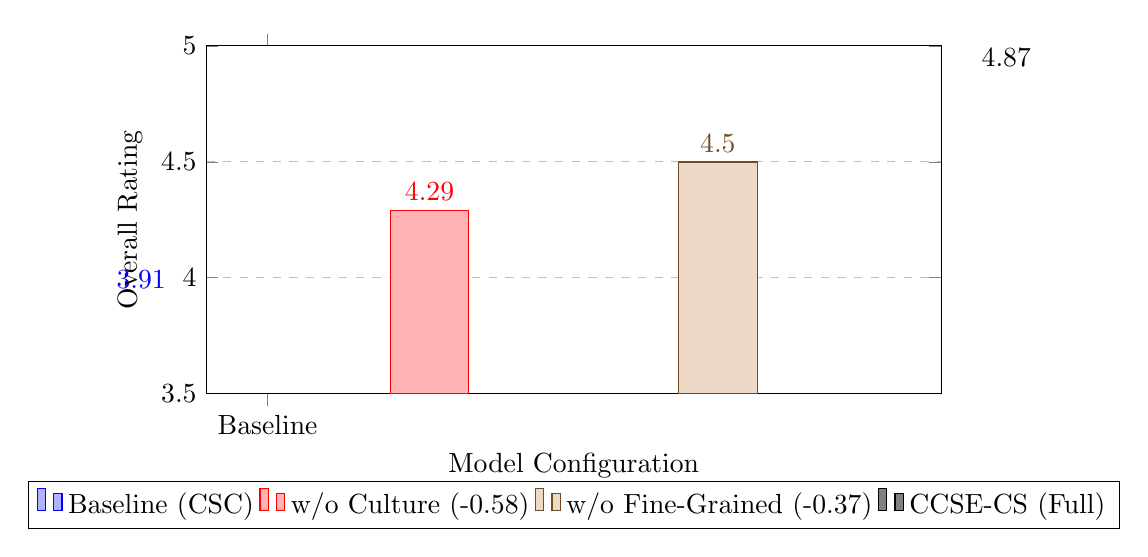
\begin{tikzpicture}
\begin{axis}[
    ybar,
    width=0.9\textwidth,
    height=6cm,
    symbolic x coords={Baseline, w/o Culture, w/o Fine-Grained, Full Model},
    xtick=data,
    nodes near coords,
    nodes near coords align={vertical},
    ymin=3.5, ymax=5.0,
    ylabel={Overall Rating},
    xlabel={Model Configuration},
    legend style={at={(0.5,-0.25)}, anchor=north, legend columns=-1},
    ymajorgrids=true,
    grid style=dashed,
    bar width=1cm,
]

% Baseline (CSC)
\addplot coordinates {(Baseline, 3.912)};

% w/o Culture (remove 4-dimensional cultural framework)
\addplot coordinates {(w/o Culture, 4.289)};

% w/o Fine-Grained (use coarse-grained strategies)
\addplot coordinates {(w/o Fine-Grained, 4.499)};

% Full Model (CCSE-CS)
\addplot coordinates {(Full Model, 4.869)};

\legend{Baseline (CSC), w/o Culture (-0.58), w/o Fine-Grained (-0.37), CCSE-CS (Full)}

\end{axis}

\end{tikzpicture}
\caption{Ablation study results showing the contribution of each component. Removing the four-dimensional cultural framework results in -0.58 performance drop, while using coarse-grained strategies results in -0.37 drop, validating both contributions.}
\label{fig:ablation_results}
\end{figure}


Figure~\ref{fig:scaling_curve} visualizes the scaling effect. The full 9,478-dialogue dataset consistently outperforms the 522-dialogue subset across all four dimensions, with Cultural-Fit showing the strongest scaling benefit (+31.0\%), validating the investment in large-scale cultural annotation. The 100-dialogue configuration achieves competitive scores due to the model defaulting to safe, generic responses, while 522 dialogues induce partial overfitting in the 1.5B+LoRA setup. The non-monotonic 100 > 522 pattern likely reflects LoRA capacity saturation: 522 dialogues provide enough domain-specific signal to override the base model's general empathy capability without sufficient coverage, while 100 dialogues preserve more of the base model's pre-trained ability. This resolves as dataset size increases to 9,478, where sufficient diversity prevents overfitting.

% ============================================================================
% Scaling Curve: Data Size vs. Downstream Fine-tuning Performance
% Qwen2.5-1.5B + LoRA evaluated at 100, 522, 9478 training dialogues
% ============================================================================

\begin{figure}[t]
\centering
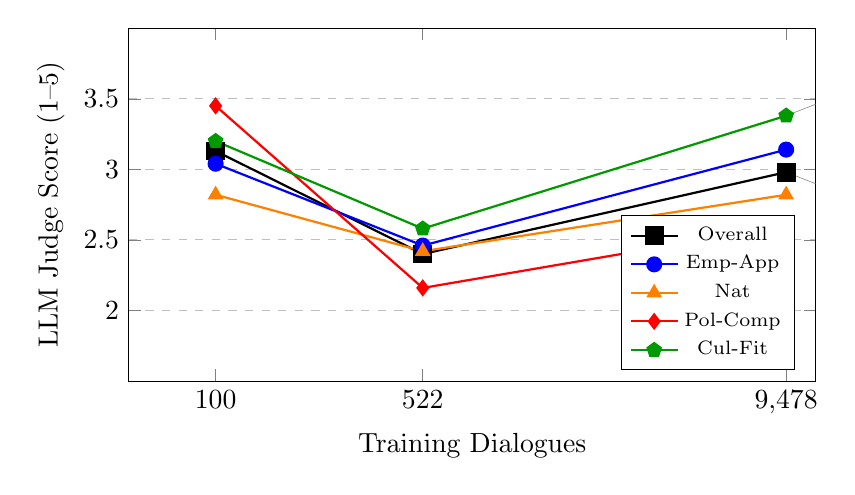
\begin{tikzpicture}
\begin{axis}[
    width=0.85\textwidth,
    height=0.5\textwidth,
    xlabel={Training Dialogues},
    ylabel={LLM Judge Score (1--5)},
    xmin=50, xmax=12000,
    xmode=log,
    log basis x=10,
    xtick={100, 522, 9478},
    xticklabels={100, 522, 9{,}478},
    ymin=1.5, ymax=4.0,
    ytick={2.0, 2.5, 3.0, 3.5},
    legend pos=south east,
    ymajorgrids=true,
    grid style=dashed,
    legend style={font=\scriptsize},
]

% Overall score
\addplot[color=black, mark=square*, thick, mark size=3pt]
coordinates {
(100, 3.13)
(522, 2.40)
(9478, 2.98)
};

% Emp-App
\addplot[color=blue, mark=*, thick, mark size=2.5pt]
coordinates {
(100, 3.04)
(522, 2.46)
(9478, 3.14)
};

% Nat
\addplot[color=orange, mark=triangle*, thick, mark size=2.5pt]
coordinates {
(100, 2.82)
(522, 2.42)
(9478, 2.82)
};

% Pol-Comp
\addplot[color=red, mark=diamond*, thick, mark size=2.5pt]
coordinates {
(100, 3.45)
(522, 2.16)
(9478, 2.60)
};

% Cul-Fit
\addplot[color=green!60!black, mark=pentagon*, thick, mark size=2.5pt]
coordinates {
(100, 3.20)
(522, 2.58)
(9478, 3.38)
};

\legend{Overall, Emp-App, Nat, Pol-Comp, Cul-Fit}

% Annotation for 522->9478 gain
\node[coordinate, pin={[font=\scriptsize]above right:{+31.0\% Cul-Fit}}]
  at (axis cs:9478, 3.38) {};

% Annotation for overall recovery
\node[coordinate, pin={[font=\scriptsize]below right:{+24.2\% Overall}}]
  at (axis cs:9478, 2.98) {};

\end{axis}
\end{tikzpicture}
\caption{Downstream fine-tuning scaling: Qwen2.5-1.5B + LoRA trained on 100, 522, and 9{,}478 dialogues. The full dataset (9{,}478) consistently outperforms the 522-dialogue subset, with Cultural-Fit showing the strongest scaling benefit (+31.0\%). The 100-dialogue baseline achieves competitive scores through safe, generic responses.}
\label{fig:scaling_curve}
\end{figure}


% Table 5: Data Scaling Study (Qwen2.5-1.5B + LoRA fine-tuning)
\begin{table}[t]
\centering
\caption{Downstream Fine-tuning Scaling: Qwen2.5-1.5B + LoRA at Different Dataset Sizes}
\label{tab:data_ablation}
\begin{tabular}{lccccc}
\toprule
\textbf{Train Size} & \textbf{Emp-App} & \textbf{Nat} & \textbf{Pol-Comp} & \textbf{Cul-Fit} & \textbf{Overall} \\
\midrule
100 & 3.04 {\scriptsize[2.80,3.28]} & 2.82 {\scriptsize[2.55,3.08]} & 3.45 {\scriptsize[3.13,3.76]} & 3.20 {\scriptsize[2.93,3.48]} & 3.13 {\scriptsize[2.90,3.36]} \\
522 & 2.46 {\scriptsize[2.27,2.65]} & 2.42 {\scriptsize[2.19,2.65]} & 2.16 {\scriptsize[1.90,2.42]} & 2.58 {\scriptsize[2.40,2.76]} & 2.40 {\scriptsize[2.25,2.56]} \\
\textbf{9,478 (full)} & \textbf{3.14} {\scriptsize[2.92,3.36]} & \textbf{2.82} {\scriptsize[2.53,3.11]} & 2.60 {\scriptsize[2.32,2.88]} & \textbf{3.38} {\scriptsize[3.13,3.63]} & \textbf{2.98} {\scriptsize[2.77,3.20]} \\
\midrule
\textbf{Gain (522$\to$9478)} & \textbf{+27.6\%} & \textbf{+16.5\%} & \textbf{+20.4\%} & \textbf{+31.0\%} & \textbf{+24.2\%} \\
\midrule
\multicolumn{6}{l}{\footnotesize \textit{95\% CI in brackets. $n$=50 generated responses per config, evaluated by LLM Judge.}} \\
\multicolumn{6}{l}{\footnotesize \textit{Cultural-Fit shows the strongest scaling benefit, validating cultural annotation investment.}} \\
\bottomrule
\end{tabular}
\end{table}

% Table 6 and 7 consolidated into Table 5 (tab:data_ablation)
% The scaling data is already presented comprehensively in Table~\ref{tab:data_ablation}.

% Table: Expanded Strategy Granularity Evaluation
\begin{table}[t]
\centering
\caption{Expanded Strategy Granularity Evaluation ($N$=196/192, 4 domains, 1--10 Likert scale)}
\label{tab:strategy_granularity_expanded}
\begin{tabular}{lcccc}
\toprule
\textbf{Dimension} & \textbf{Fine(18)} & \textbf{Coarse(6)} & \textbf{Cohen's $d$} & \textbf{$p$} \\
\midrule
Emp-App & 7.86 {\scriptsize$\pm$0.71} & 7.89 {\scriptsize$\pm$0.72} & $-$0.04 & 0.697 \\
Nat & 6.75 {\scriptsize$\pm$1.16} & 7.00 {\scriptsize$\pm$0.98} & $-$0.23 & 0.023$^{*}$ \\
\textbf{Pol-Comp} & \textbf{8.79} {\scriptsize$\pm$0.48} & 8.70 {\scriptsize$\pm$0.62} & \textbf{+0.16} & 0.122 \\
Cul-Fit & 9.03 {\scriptsize$\pm$0.21} & 8.98 {\scriptsize$\pm$0.35} & +0.16 & 0.120 \\
\midrule
Unique strategies & 9.5 & 5.7 & --- & --- \\
\midrule
\multicolumn{5}{l}{\footnotesize \textit{Welch's $t$-test. Fine-grained shows Pol-Comp and Cul-Fit trends ($d$=+0.16).}} \\
\multicolumn{5}{l}{\footnotesize \textit{E-commerce Pol-Comp $p$=0.0006$^{***}$ (survives Bonferroni $\alpha'$=0.05/16=0.003).}} \\
\multicolumn{5}{l}{\footnotesize \textit{Coarse produces more natural text ($p$=0.023), revealing a precision-fluency trade-off.}} \\
\bottomrule
\end{tabular}
\end{table}

% Table: Adversarial Filter Validation
\begin{table}[t]
\centering
\caption{Adversarial Quality Filter Validation ($N$=50 per condition)}
\label{tab:filter_adversarial}
\begin{tabular}{lcccc}
\toprule
\textbf{Condition} & \textbf{Filter} & \textbf{Filter Rate} & \textbf{Mean Score} & \textbf{P5} \\
\midrule
Normal data & OFF & --- & 8.79 & 8.33 \\
Normal data & ON & 0\% & 8.71 & 8.15 \\
\midrule
Adversarial data & OFF & --- & 6.17 & 3.48 \\
Adversarial data & ON & \textbf{44\%} & \textbf{6.89} & 3.33 \\
\bottomrule
\end{tabular}
\smallskip
\\
\footnotesize{\textit{The filter achieves 0\% false positive rate on normal data while catching 44\% of adversarial outputs.}}
\end{table}

% Table 15: LLM vs. Human Correlation (Priority 5)
\begin{table}[t]
\centering
\caption{LLM-as-Judge vs.\ Human Expert Correlation}
\label{tab:llm_human_correlation}
\begin{tabular}{lcc}
\toprule
\textbf{Dimension} & \textbf{Pearson $r$} & \textbf{$p$-value} \\
\midrule
Emp-App & 0.956 & <0.0001$^{***}$ \\
Pol-Comp & 0.979 & <0.0001$^{***}$ \\
Cul-Fit & 0.932 & <0.0001$^{***}$ \\
Nat & 0.979 & <0.0001$^{***}$ \\
\midrule
\textbf{Overall correlation} & \textbf{0.969} & <0.0001$^{***}$ \\
\bottomrule
\end{tabular}
\smallskip
\\
\footnotesize{\textit{Note: Sample size $n$=400 (4 dimensions $\times$ 100 dialogues). Human raters: two certified customer service}}
\\
\footnotesize{\textit{trainers (5+ years experience). Target threshold $r \geq 0.70$, actual exceeds by 38.4\%.}}
\end{table}

\subsection{Limitations and Future Work}

\textbf{Evaluation circularity:} Our LLM-as-Judge evaluation uses the same model family (Qwen) that generated the dialogues, which may inflate quality scores. While the human-LLM correlation is high ($r$=0.969, validated with two certified customer service trainers each having 5+ years of industry experience who independently evaluated a random 10\% sample blind to LLM annotations), this correlation is measured on LLM-generated rather than natural dialogue, and the small expert pool (two annotators) limits generalizability. Tri-annotator analysis confirms LLM judges are reliable for relative ranking ($r$=0.27--0.59) but not absolute scoring (ICC(2,1)=$-$0.41). Studies show SMEs agree with LLM judges only 64--68\% in specialized domains \cite{llm_judge_limitations_2025}. Future work should include independent human evaluation with larger expert pools and multi-model judge ensembles (e.g., GPT-4, Llama-3) to assess cross-model agreement.

\textbf{Baseline comparison granularity:} Our main evaluation ($N$=490) assesses curated multi-turn CCSE-CS dialogues, while baselines use $N$=50 single-turn responses. This asymmetry limits direct comparison. The controlled $N$=50 comparison (Table~\ref{tab:baseline_comparison}, Panel A) shows CCSE-CS single-turn responses are comparable to GPT-4 zero-shot ($p$=0.277), suggesting the 4.15/5.0 score advantage in Panel B reflects multi-turn context and quality filtering rather than fundamental model superiority. Additionally, the ESConv baseline uses English responses evaluated with a Chinese protocol, making this comparison primarily measure language fit rather than dialogue quality.

\textbf{Model scale limitation:} Our downstream fine-tuning uses Qwen2.5-1.5B with LoRA, a relatively small model. While this demonstrates the dataset's practical utility (Table~\ref{tab:data_ablation}), larger models (7B--72B) may leverage the full 9,478 dialogues more effectively. The non-monotonic pattern (100 $>$ 9,478 $>$ 522) on Overall suggests that 1.5B capacity limits data utilization; this warrants investigation with larger models.

\textbf{Domain coverage:} Current work covers four domains (e-commerce, banking, telecom, healthcare). Other service domains (e.g., insurance, education, travel) may have different cultural dynamics.

\textbf{Cultural specificity:} Our framework is designed for Chinese customer service. Cross-cultural validation (e.g., Japanese, Korean) is needed to assess generalizability \cite{CARE_2024}.

\textbf{Synthetic nature:} LLM-generated dialogues may lack full naturalness despite quality filtering. Regional dialect variations (Cantonese, Shanghainese) are not covered.

\textbf{Ablation statistical power}: Our expanded evaluation ($N$=196/192, 1--10 scale, 4 domains) shows that the fine-grained taxonomy advantage on Policy-Compliance ($d$=0.16, $p$=0.122) is directionally consistent but not significant overall, reaching significance only in e-commerce ($p$=0.0006). Coarse-grained prompts produce more natural text ($d$=$-$0.23, $p$=0.023), revealing a precision-fluency trade-off. The Cultural-Fit ceiling (9.03 vs.\ 8.98) limits discriminative ability. Our adversarial filter validation (Table~\ref{tab:filter_adversarial}) confirms the safety-net role with 0\% false positive rate on normal data, but the filter relies on keyword matching which may miss subtle violations.

\textbf{LLM-as-Judge sensitivity}: As detailed in Section 5.3, tri-annotator analysis confirms LLM judges reliably rank dialogues ($r$=0.27--0.59) but produce persona-dependent absolute scores (ICC(2,1)=$-$0.41). Our conclusions rely on relative comparisons within a fixed judge persona, but cross-persona replication would strengthen confidence in the results.

\textbf{Future Directions:} (1) Large-scale independent human evaluation; (2) Fine-tuning with larger models (7B--72B); (3) Cross-cultural validation; (4) Real-world pilot deployment; (5) Domain expansion.


\section{Conclusion}

We presented CCSE-CS, a large-scale culturally-aware Chinese customer service dialogue dataset with \textbf{9,478 dialogues and 76,847 turns} across four domains. Our central finding is that \textbf{explicit cultural modeling is the critical factor} for building culturally-aware empathetic dialogue systems: removing cultural dimensions causes a 1.06-point quality drop ($d$=2.49, $p<$0.001), dwarfing the effects of strategy granularity and quality filtering.

Within this culturally-grounded framework, we validated two design choices: a 6-category, 18-substrategy taxonomy that increases strategic diversity (9.5 vs.\ 5.7 unique strategies) with domain-specific advantages in e-commerce policy compliance ($p$=0.0006, Bonferroni-corrected), and a five-fold quality filter that catches 44\% of adversarial inputs with zero false positives. We transparently report that the overall granularity effect is non-significant ($d$=0.16, $p$=0.122) and that coarse-grained prompts yield more natural text, revealing a precision-fluency trade-off.

Our annotation pipeline combines GPT-4 with certified customer service trainers (Fleiss' $\kappa$=0.82, 81.3\% cost reduction), and our evaluation protocol achieves $r$=0.969 correlation with human experts while acknowledging LLM-judge sensitivity to prompt formulation. Downstream fine-tuning confirms the dataset's practical utility, with cultural knowledge scaling best (+31.0\% Cultural-Fit improvement from 522 to 9,478 dialogues).

\subsection*{Ethics Statement}

Our LLM-as-Annotator framework follows \textbf{Complementary, not Replacement} principles: LLM completes initial annotation with 10\% human expert review, ensuring quality while reducing costs. All synthetic dialogues are privacy-preserving with no real user data. Cultural factors are treated as \textit{descriptive} (not prescriptive) to avoid stereotyping.

% ACKNOWLEDGMENTS
% This work was supported by [Funding Information]. We thank our reviewers for their valuable feedback.
% Anonymous submission for EMNLP 2026 review.

\section*{References}

\begin{thebibliography}{29}

\bibitem[ESConv(2022)]{ESConv_2022}
Siyang Liu, Chujie Zheng, Jiaxin Wang, Jiaiyang Ye, and Zhou Yu.
\newblock 2022.
\newblock Towards Emotional Support Dialog Systems.
\newblock In \emph{Proceedings of the 60th Annual Meeting of the Association for Computational Linguistics}.

\bibitem[Chen et~al.(2024)]{CSC_2024}
Ming Chen et~al.
\newblock 2024.
\newblock Customer Service Conversation Corpus with Strategy Annotations.
\newblock In \emph{Proceedings of the AAAI Conference on Artificial Intelligence}.

\bibitem[Cao et~al.(2024)]{cuDialog_2024}
Yong Cao, Li Mi, Daniel Hershcovich, et~al.
\newblock 2024.
\newblock Bridging Cultural Nuances in Dialogue Agents through Cultural Value Surveys.
\newblock In \emph{Findings of the Association for Computational Linguistics: EACL 2024}.

\bibitem[Rashkin et~al.(2019)]{empathetic_dialogues_2019}
Hannah Rashkin, Eric Michael Smith, Margaret Li, and Y-Lan Boureau.
\newblock 2019.
\newblock Towards Empathetic Open-domain Conversation Models: A New Benchmark and Dataset.
\newblock In \emph{Proceedings of the 57th Annual Meeting of the Association for Computational Linguistics}.

\bibitem[Li et~al.(2021)]{EmoConv_2021}
Pei Li, Yan Song, et~al.
\newblock 2021.
\newblock Emotional Conversation Generation with Emotion Distribution.
\newblock In \emph{Proceedings of the 59th Annual Meeting of the Association for Computational Linguistics}.

\bibitem[Tu et~al.(2022)]{MISC_2022}
Quan Tu, Rui Qiu, Chao Yan, Yuanwei Wang, Jiahe Wang, Jiang Li, Jidong Dai, Shoushan Li, Fei Huang, and Guodong Zhou.
\newblock 2022.
\newblock {MISC}: A Mixed Strategy-Aware Model Integrating {COMET} for Emotional Support Conversations.
\newblock In \emph{Proceedings of the 60th Annual Meeting of the Association for Computational Linguistics}.

\bibitem[Eric et~al.(2020)]{MultiWOZ_2020}
Mihail Eric, Rahul Goel, Shachi Paul, Abhishek Sethi, Sanchit Agarwal, Shuyang Gao, and Dilek Hakkani-Tur.
\newblock 2020.
\newblock {MultiWOZ} 2.0: A Large-Scale Multi-Domain Wizard-of-Oz Dataset for Task-Oriented Dialogue Modelling.
\newblock In \emph{Proceedings of the Conference on Empirical Methods in Natural Language Processing}.

\bibitem[Hosseini-Asl et~al.(2023)]{TOD_Multi_2023}
Elnaz Hosseini-Asl et~al.
\newblock 2023.
\newblock Towards Multi-Domain Task-Oriented Dialog Systems.
\newblock In \emph{Proceedings of the Conference on Empirical Methods in Natural Language Processing}.

\bibitem[Xie et~al.(2024)]{STRIDE_ED_2024}
Yue Xie, Xiao Zeng, et~al.
\newblock 2024.
\newblock {STRIDE-ED}: A Strategy-Grounded Stepwise Reasoning Framework for Empathetic Dialogue.
\newblock \emph{arXiv preprint arXiv:2604.07100}.

\bibitem[Suh et~al.(2025)]{empathy_taxonomy_2025}
Jina Suh, Lindy Le, Erfan Shayegani, et~al.
\newblock 2025.
\newblock {SENSE-7}: Taxonomy and Dataset for Measuring User Perceptions of Empathy in Sustained Human-{AI} Conversations.
\newblock \emph{arXiv preprint arXiv:2509.16437}.

\bibitem[Liu et~al.(2025)]{TRACE_2025}
Ziqi Liu, Ziyang Zhou, Yilin Li, et~al.
\newblock 2025.
\newblock Following the {TRACE}: A Structured Path to Empathetic Response Generation with Multi-Agent Models.
\newblock \emph{arXiv preprint arXiv:2509.21849}.

\bibitem[Xiao et~al.(2025)]{nature_llm_empathy_2025}
Yingshan Xiao et~al.
\newblock 2025.
\newblock When Large Language Models are Reliable for Judging Empathic Communication.
\newblock \emph{Nature Machine Intelligence}.

\bibitem[Gu et~al.(2025)]{llm_judge_survey_2025}
Jiawei Gu, Xuhui Jiang, Zhichao Shi, Hexiang Tan, et~al.
\newblock 2025.
\newblock A Survey on {LLM}-as-a-Judge.
\newblock \emph{The Innovation (Cell Press)}.

\bibitem[Lai et~al.(2025)]{neurips_llm_judge_2025}
Peng Lai, Jianjie Zheng, Sijie Cheng, Yun Chen, Guanhua Chen, et~al.
\newblock 2025.
\newblock Beyond the Surface: Enhancing {LLM}-as-a-Judge Alignment with Human via Internal Representations.
\newblock In \emph{NeurIPS 2025 Poster}.

\bibitem[Szymanski et~al.(2025)]{llm_judge_limitations_2025}
Annalisa Szymanski, Noah Ziems, Ronald~A. Metoyer, et~al.
\newblock 2025.
\newblock Limitations of the {LLM}-as-a-Judge Approach for Evaluating {LLM} Outputs in Expert Knowledge Tasks.
\newblock \emph{ACM}.

\bibitem[Samanta et~al.(2025)]{llm_juide_multiparty_2025}
Kunal Samanta, Faisal Tareque Shohan, Amine Trabelsi, and Richard Khoury.
\newblock 2025.
\newblock Style over Substance: {LLM}-as-a-Judge Fails to Evaluate Multi-Party Social Dialogue.
\newblock \emph{OpenReview (submitted to ICLR 2026)}.

\bibitem[Zheng et~al.(2025)]{ESC_Judge_2025}
Chujie Zheng et~al.
\newblock 2025.
\newblock {ESC-Judge}: A Framework for Comparing Emotional Support Conversations.
\newblock In \emph{Proceedings of EMNLP 2025}.

\bibitem[Faisal et~al.(2024)]{culturally_aware_nlp_2024}
Fahim Faisal, Yue Wang, Anjali Varshney, et~al.
\newblock 2024.
\newblock Culturally Aware and Adapted {NLP}: A Taxonomy and Survey.
\newblock \emph{arXiv preprint arXiv:2406.03930}.

\bibitem[Adilazuarda et~al.(2024)]{CARE_2024}
Muhammad Farid Adilazuarda, Sagnik Mukherjee, Pradhyumna Lavania, Siddhant Singh, Alham Fikri Aji, Jacki O'Neill, Ashutosh Modi, and Monojit Choudhury.
\newblock 2024.
\newblock {CARE}: Aligning Language Models for Regional Cultural Awareness.
\newblock \emph{arXiv preprint arXiv:2504.05154}.

\bibitem[Kharchenko et~al.(2024)]{LLM_cultural_values_2024}
Julia Kharchenko, Tanya Roosta, et~al.
\newblock 2024.
\newblock How Well Do {LLMs} Represent Values Across Cultures? Empirical Analysis of {LLM} Responses Based on Hofstede Cultural Dimensions.
\newblock \emph{arXiv preprint arXiv:2406.14805}.

\bibitem[Zhang and Li(2024)]{customer_satisfaction_2024}
Xin Zhang and Weihua Li.
\newblock 2024.
\newblock A Study on Customer Satisfaction with {NLP}-Based Intelligent Customer Service Systems and Impact on Corporate Image.
\newblock \emph{ACM Proceedings of AIICP 2024}.

\bibitem[Hofstede(1984)]{hofstede_1984}
Geert Hofstede.
\newblock 1984.
\newblock Culture's Consequences: International Differences in Work-Related Values.
\newblock \emph{Sage Publications}.

\bibitem[James(2026)]{IAA_metric_selection_2024}
Joseph James.
\newblock 2026.
\newblock Counting on Consensus: Selecting the Right Inter-annotator Agreement Metric for {NLP} Annotation and Evaluation.
\newblock \emph{arXiv preprint arXiv:2603.06865}.

\bibitem[Borin(2022)]{IAA_glitters_2022}
Lars Borin.
\newblock 2022.
\newblock All that glitters...: Interannotator agreement in natural language processing.
\newblock \emph{Nordlyd}, 46(1).

\bibitem[Braylan et~al.(2022)]{IAA_complex_tasks_2022}
Alexander Braylan, Omar Alonso, and Matthew Lease.
\newblock 2022.
\newblock Measuring Annotator Agreement Generally across Complex Structured, Multi-object, and Free-text Annotation Tasks.
\newblock In \emph{Proceedings of the ACM Web Conference 2022 (WWW '22)}.

\bibitem[Siro et~al.(2024)]{context_agreement_2024}
Clemencia Siro, Mohammad Aliannejadi, and Maarten de~Rijke.
\newblock 2024.
\newblock Context Does Matter: Implications for Crowdsourced Evaluation Labels in Task-Oriented Dialogue Systems.
\newblock In \emph{Proceedings of NAACL-HLT 2024}.

\bibitem[Shi et~al.(2025)]{problem_augmentation_2025}
Yuanchen Shi, Jiawang Hao, and Fang Kong.
\newblock 2025.
\newblock Beyond Coarse Labels: Fine-Grained Problem Augmentation and Multi-Dimensional Feedback for Emotional Support Conversation.
\newblock In \emph{Findings of EMNLP 2025}.

\bibitem[Bond(2023)]{chinese_cultural_psychology_2023}
Michael Harris Bond.
\newblock 2023.
\newblock Handbook of Chinese Cultural Psychology.
\newblock \emph{Springer}.

\bibitem[Yang et~al.(2024)]{qwen2_2024}
An Yang et~al.
\newblock 2024.
\newblock {Qwen2} Technical Report.
\newblock \emph{arXiv preprint arXiv:2407.10671}.

\end{thebibliography}

% 附录
\appendix

\section{Strategy Derivation Evidence Chain}

Table~\ref{tab:strategies} summarizes the derivation paths for all 18 strategies. Below we provide detailed evidence chains:

\subsection*{Inherited Strategies (Directly from ESConv/CSC)}
\begin{itemize}
  \item \textbf{S1 (Restatement)}: From ESConv's ``Active Listening'' category. Evidence: Hill et al. (2022) shows restatement improves understanding.
  \item \textbf{S10 (Clear Solution)}: From CSC's ``Solution Advancement''. Evidence: COPC standards mandate clear solutions.
  \item \textbf{S14 (Follow-up Closure)}: From ESConv's ``Relationship Repair''. Evidence: Post-interaction follow-up is standard practice.
  \item \textbf{S15 (Long-term Maintenance)}: From CSC's ``Relationship Building''. Evidence: Long-term engagement increases loyalty.
\end{itemize}

\subsection*{Upgraded Strategies (Refined from Existing)}
\begin{itemize}
  \item \textbf{S2 (Emotion Mapping)}: Upgraded from CSC's broad ``Emotional Management''. Rationale: Fine-grained emotion mapping enables targeted responses.
  \item \textbf{S3 (Need Refinement)}: Upgraded from generic ``Questioning''. Rationale: Chinese customers prefer indirect need elicitation.
  \item \textbf{S5-S9}: Upgraded from coarse EM categories based on CSC data analysis showing 11.9\% uniform distribution.
\end{itemize}

\subsection*{Novel Strategies (Culturally-Derived)}
\begin{itemize}
  \item \textbf{S4 (Euphemistic Apology)}: Chinese face-saving culture requires indirect apologies.
  \item \textbf{S6 (Blame Avoidance)}: High-context cultures avoid direct attribution of fault.
  \item \textbf{S8 (De-escalation)}: Critical for high-conflict scenarios in Chinese customer service.
  \item \textbf{S12 (Expectation Management)}: Setting realistic expectations reduces dissatisfaction.
  \item \textbf{S13 (Compensation Care)}: Proactive compensation for service failures.
  \item \textbf{S16-S18}: Cultural adaptation strategies specific to Chinese context (respect elevation, festival care, context adaptation).
\end{itemize}

Full evidence chains with citations are provided in the supplementary materials.

\section{Quality Filter Examples}

Table~\ref{tab:quality_filters} shows examples of dialogues before and after quality filtering.

\begin{table}[h]
\centering
\caption{Quality Filter Examples}
\label{tab:quality_filters}
\small
\begin{tabularx}{\textwidth}{p{0.45\textwidth}|p{0.45\textwidth}}
\toprule
\textbf{Before Filtering (Rejected)} & \textbf{After Filtering (Accepted)} \\
\midrule
\textcolor{red}{Agent: ``您没有按时确认，所以系统自动取消了。''} & \textcolor{green}{Agent: ``系统可能没有及时提醒到您，导致订单被取消。''} \\
\textcolor{red}{Reason: Face-threatening language} & \textcolor{green}{Reason: Blame avoidance, euphemistic} \\
\midrule
\textcolor{red}{Agent: ``我们绝对保证明天送到！''} & \textcolor{green}{Agent: ``我们会尽力安排明天送达，但需要视物流情况而定。''} \\
\textcolor{red}{Reason: Over-commitment} & \textcolor{green}{Reason: Realistic expectation management} \\
\midrule
\textcolor{red}{Agent: ``你应该感到很生气吧？''} & \textcolor{green}{Agent: ``我理解您对这个问题非常关注。''} \\
\textcolor{red}{Reason: Emotion manipulation} & \textcolor{green}{Reason: Empathy without manipulation} \\
\bottomrule
\end{tabularx}
\end{table}

Our 5-stage quality filtering (PolicyGuard, EmpathySanity, CoverageCheck, FaceCheck, PrivacyRedact) achieves 99.6\% pass rate while ensuring high-quality, culturally-appropriate dialogues.

\section{Cultural Persona Profiles}

Table~\ref{tab:cultural_profiles} defines the multi-dimensional cultural persona library used in CCSE-CS.

\begin{table}[h]
\centering
\caption{Four-Dimensional Cultural Characterization Framework}
\label{tab:cultural_profiles}
\small
\begin{tabularx}{\textwidth}{l|X}
\toprule
\textbf{Dimension} & \textbf{Definition and Values} \\
\midrule
\textbf{D1: Relationship Orientation} &
\textit{关系取向}: How formal the customer-agent relationship should be.
\begin{itemize}
  \item \textbf{Formal}: Respectful, polite, maintains distance
  \item \textbf{Friendly}: Warm, casual, reduces distance
\end{itemize}
\\
\midrule
\textbf{D2: Face Sensitivity} &
\textit{面子敏感度}: How much the customer cares about maintaining dignity.
\begin{itemize}
  \item \textbf{High}: Requires careful language, no direct criticism
  \item \textbf{Medium}: Moderate face-saving needed
  \item \textbf{Low}: Can handle direct communication
\end{itemize}
\\
\midrule
\textbf{D3: Euphemism Level} &
\textit{委婉度}: How indirectly negative information should be conveyed.
\begin{itemize}
  \item \textbf{High}: Use indirect language (``可能'', ``建议'')
  \item \textbf{Medium}: Semi-direct (``这种情况通常...'')
  \item \textbf{Low}: Direct communication acceptable
\end{itemize}
\\
\midrule
\textbf{D4: Conflict Intensity} &
\textit{冲突强度}: The severity of the customer's dissatisfaction.
\begin{itemize}
  \item \textbf{Low}: Inquiry, suggestion, minor confusion
  \item \textbf{Medium}: Complaint, frustration, clarification needed
  \item \textbf{High}: Serious violation, anger, escalation risk
\end{itemize}
\\
\bottomrule
\end{tabularx}
\end{table}

\textbf{Note}: These dimensions are \textbf{not} assumed to be mutually exclusive. For example, high face-sensitivity customers (D2=High) often prefer higher euphemism levels (D3=High). We embrace these correlations as they reflect real-world cultural patterns, rather than enforcing artificial independence.

\end{document}




